\documentclass[10pt]{article}
\usepackage[utf8]{inputenc}
\usepackage[spanish]{babel}
\usepackage{amsmath}
\usepackage{amsfonts}
\usepackage{amssymb}
\usepackage{graphics}
\usepackage{graphicx}
\usepackage[left=2cm,right=2cm,top=2cm,bottom=2cm]{geometry}
\usepackage{imakeidx}
\makeindex[columns=3, title=Alphabetical Index, intoc]
\usepackage{listings}
\usepackage{multicol}
\usepackage{changepage}
\usepackage{float}
\usepackage{cite}
\usepackage{url}
\usepackage{hyperref}
\usepackage{pdflscape}
\usepackage[document]{ragged2e}
\usepackage{xcolor,colortbl}

\hypersetup{
    colorlinks=true,
    linkcolor=blue,
    filecolor=magenta,
    urlcolor=blue,
}

\definecolor{Red}{rgb}{0.7,0,0}
\definecolor{LightCyan}{rgb}{0.88,1,1}
\definecolor{AquaCyan}{rgb}{0.2,1,0.5}
\definecolor{Gray}{gray}{0.85}
\definecolor{DarkBlue}{rgb}{0.1,0.1,0.5}

\definecolor{codegreen}{rgb}{0,0.6,0}
\definecolor{codegray}{rgb}{0.5,0.5,0.5}
\definecolor{codepurple}{rgb}{0.58,0,0.82}
\definecolor{backcolour}{rgb}{0.95,0.95,0.92}

\lstdefinestyle{mystyle}{
    backgroundcolor=\color{backcolour},
    commentstyle=\color{codegreen},
    keywordstyle=\color{magenta},
    numberstyle=\tiny\color{codegray},
    stringstyle=\color{codepurple},
    basicstyle=\ttfamily\footnotesize,
    breakatwhitespace=false,
    breaklines=true,
    captionpos=b,
    keepspaces=true,
    numbers=left,
    numbersep=5pt,
    showspaces=false,
    showstringspaces=false,
    showtabs=false,
    tabsize=3
}
\def\fillandplacepagenumber{%
 \par\pagestyle{empty}%
 \vbox to 0pt{\vss}\vfill
 \vbox to 0pt{\baselineskip0pt
   \hbox to\linewidth{\hss}%
   \baselineskip\footskip
   \hbox to\linewidth{%
     \hfil\thepage\hfil}\vss}}
\lstset{style=mystyle}

\lstset{
     literate=%
         {á}{{\'a}}1
         {í}{{\'i}}1
         {é}{{\'e}}1
         {ý}{{\'y}}1
         {ú}{{\'u}}1
         {ó}{{\'o}}1
         {ñ}{{\~n}}1
}


\title{Escuela Superio de Cómputo\\Instituto Politécnico Nacional\\Administración de Servicios en Red\\Practica 3\\Curso impartido por: Ricardo Martinez Rosales}

\author{Adrian González Pardo}

\date{\today}

\newcommand\tab[1][1cm]{\hspace*{#1}}

\begin{document}
\maketitle
\section{Descripción y Desarrollo}
Para desarrollar esta practica, previamente se estudio y se leyo acerca de los siguientes temas:
\begin{itemize}
  \item Protocolos de Enrutamiento Estatico y Dinamico (RIP,OSPF)
  \item Enrutamiento multiple de resdistribución en protocolos Dinamicos
  \item Configuración de usuarios y de sesiones remotas
  \item Conexión SSH o Telnet vía Python
\end{itemize}
Para realizar esta practica las precondiciones de la misma es inicialmente configurar los routers, levantar al menos un usuario en telnet o ssh para conexión remota en todos los routers (Considerarlo usuario por defecto), encender y configurar las interfaces necesarias para trabajar. guardar el archivo y continuar con la aplicación
\subsection{Aplicación desarrollada}
\begin{center}
  \lstinputlisting[language=Python]{script/main.py}
  \lstinputlisting[language=Python]{script/module\_scan.py}
  \lstinputlisting[language=Python]{script/detecta.py}
  \lstinputlisting[language=Python]{script/ssh\_connect.py}
\end{center}
De modo que estos scripts hacen toda la aplicación y posible la solución de la configuración de los routers

\section{Parte de demostración}
Para la demostración de como se desarrollo y una pequeña explicación se grabo un vídeo que se puede ver \underline{\href{https://youtu.be/bnYkfwaPU50}{aquí}} destacando y pidiendo disculpa por la cantidad de sueño que se expresa directamente o indirectamente durante la grabación y presentación.

Por otro lado se anexan imagenes de las pruebas y del como se realizaron:
\begin{center}
  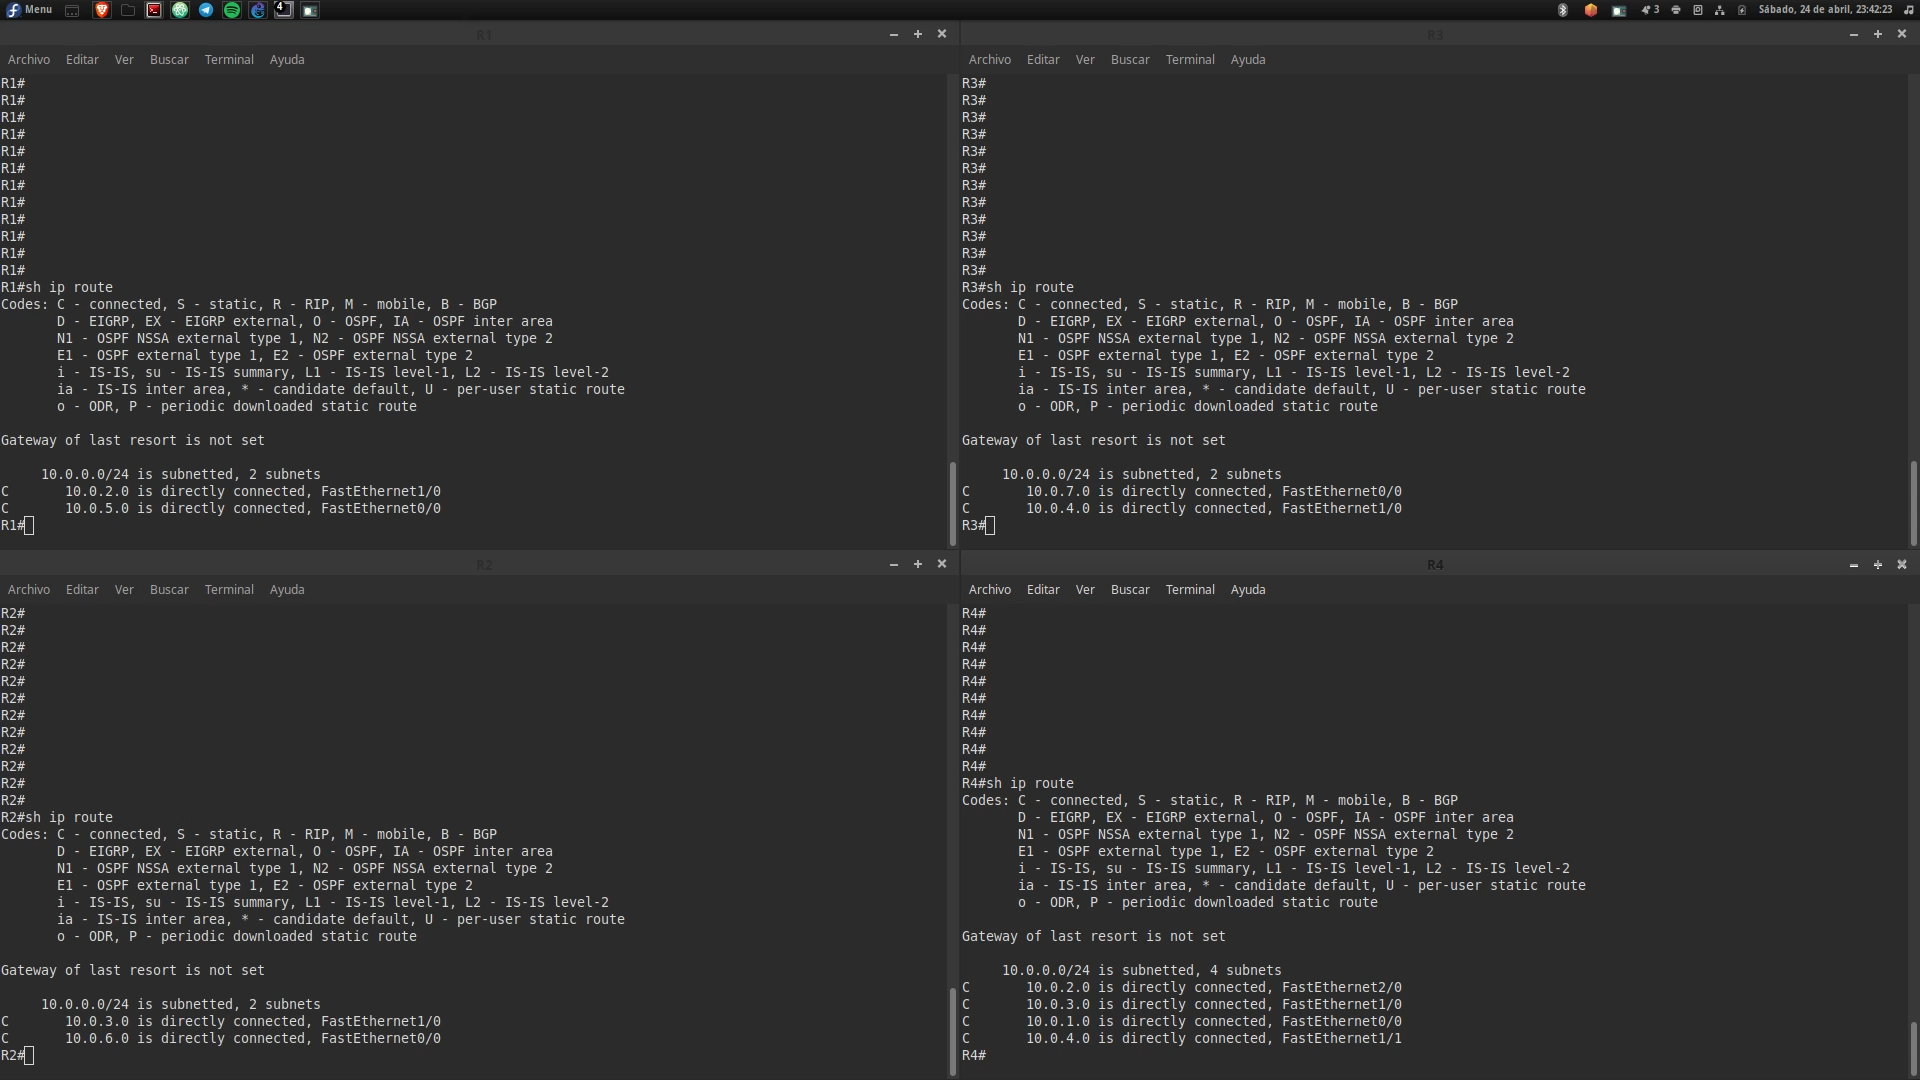
\includegraphics[scale=0.5]{imgs/1.png}\\
  \textit{Figura 1: Tablas de enrutamiento sin configurar}
  \\
  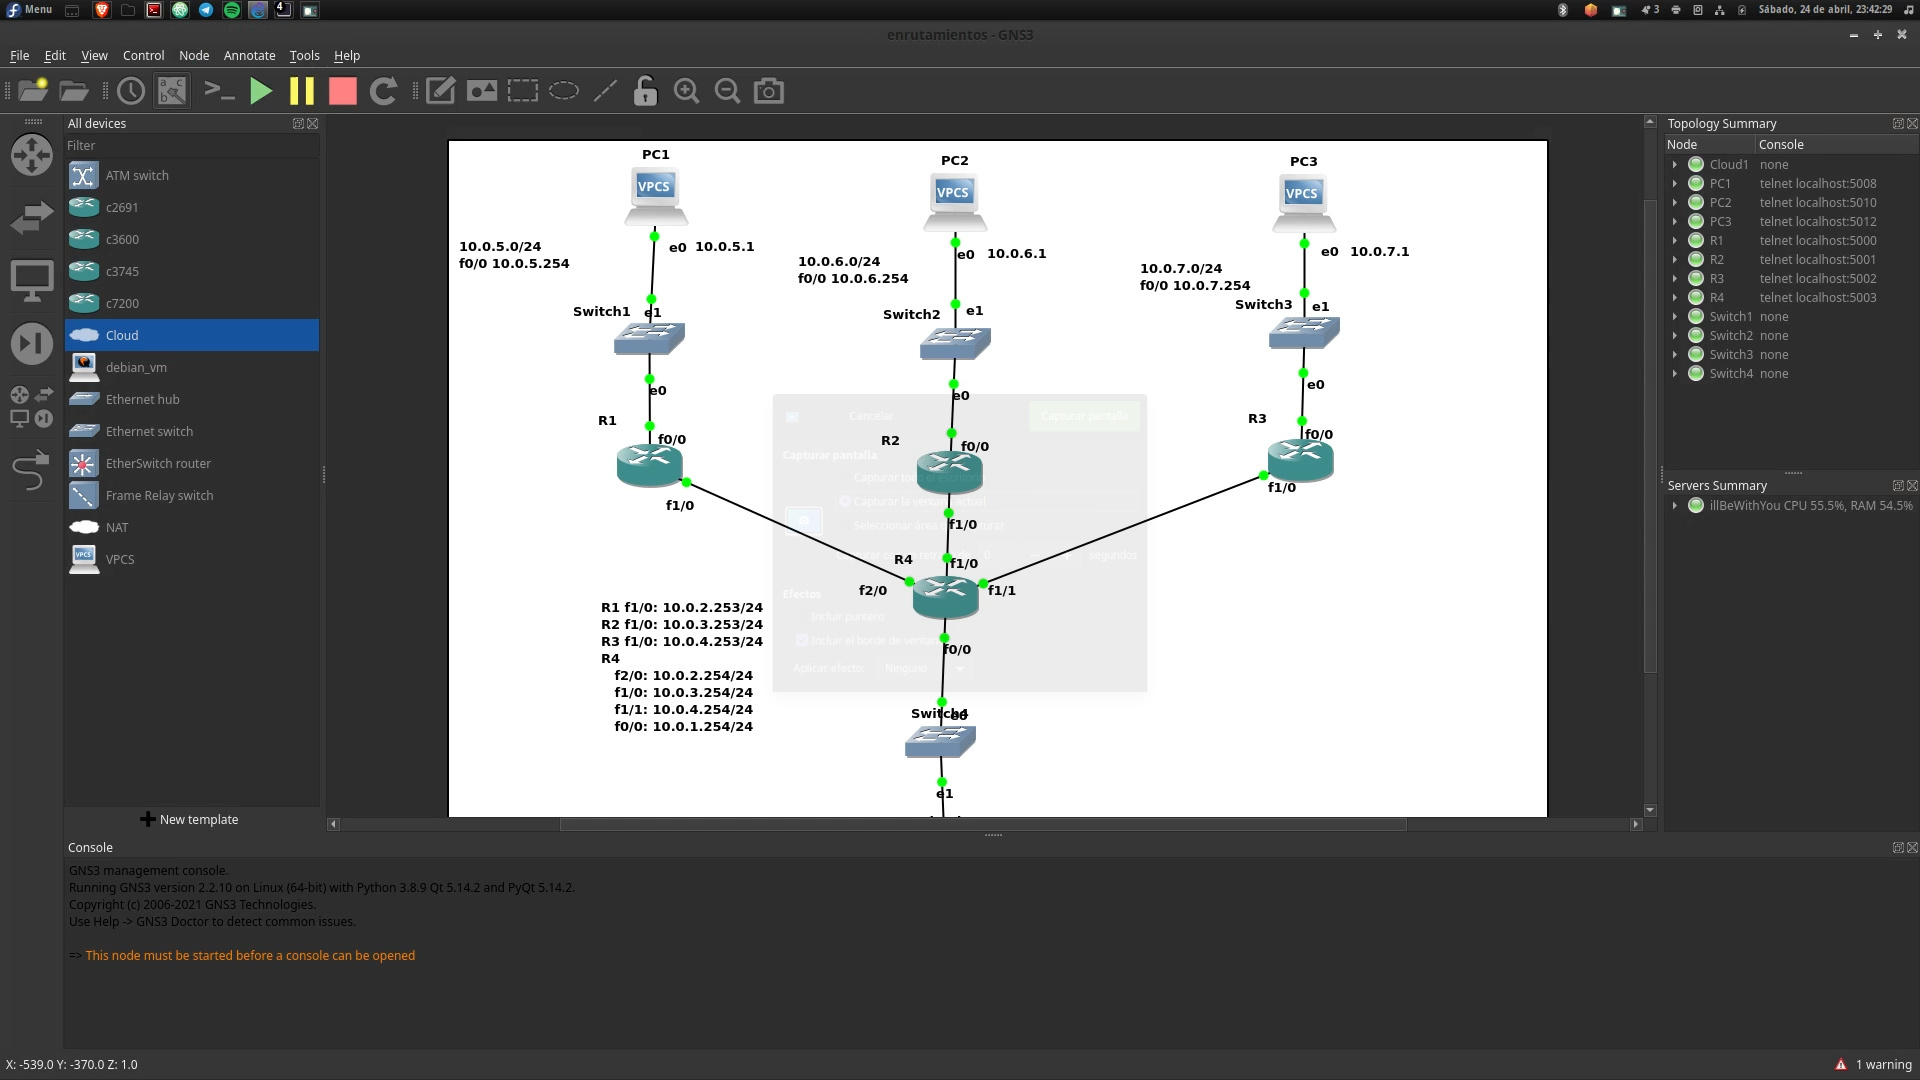
\includegraphics[scale=0.5]{imgs/2.png}\\
  \textit{Figura 2: Topología de red}\\
  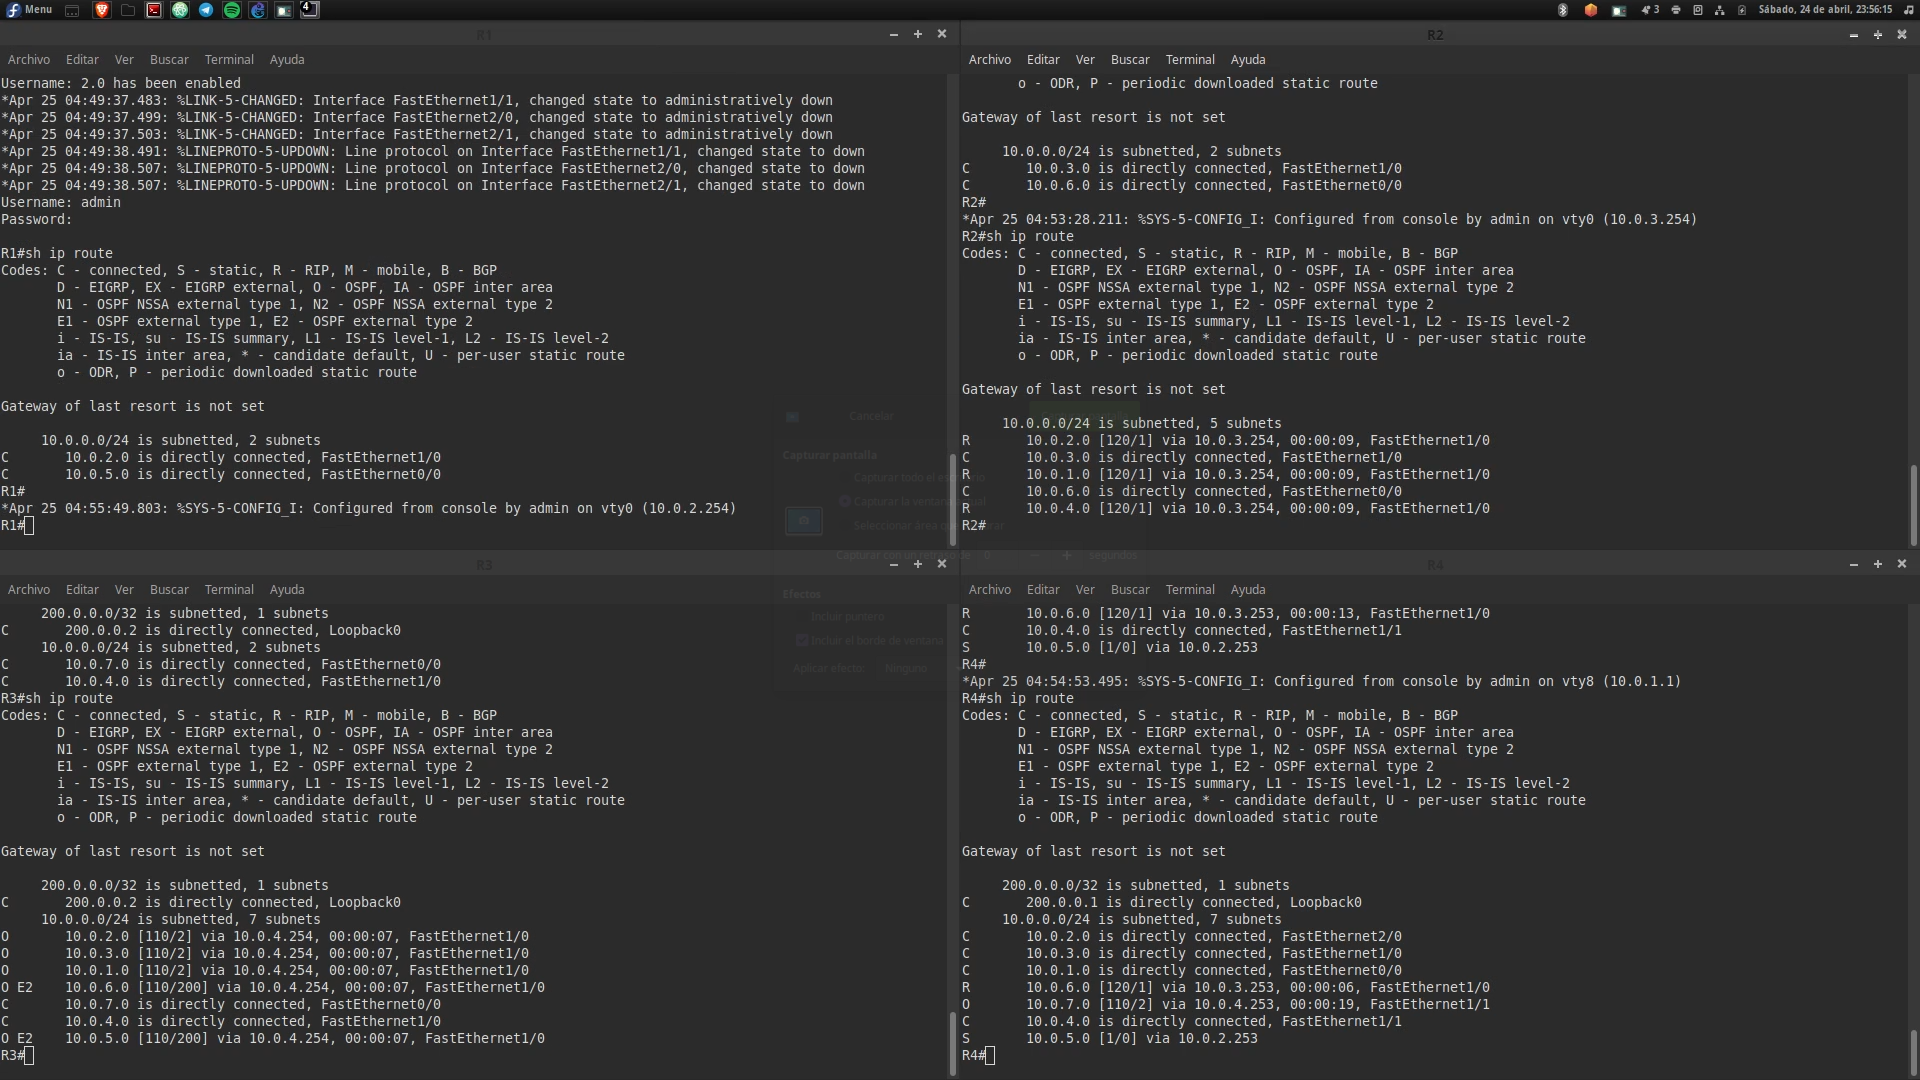
\includegraphics[scale=0.5]{imgs/3.png}\\
  \textit{Figura 3: Tablas de enrutamiento despues de ejecución del script}
  \\
  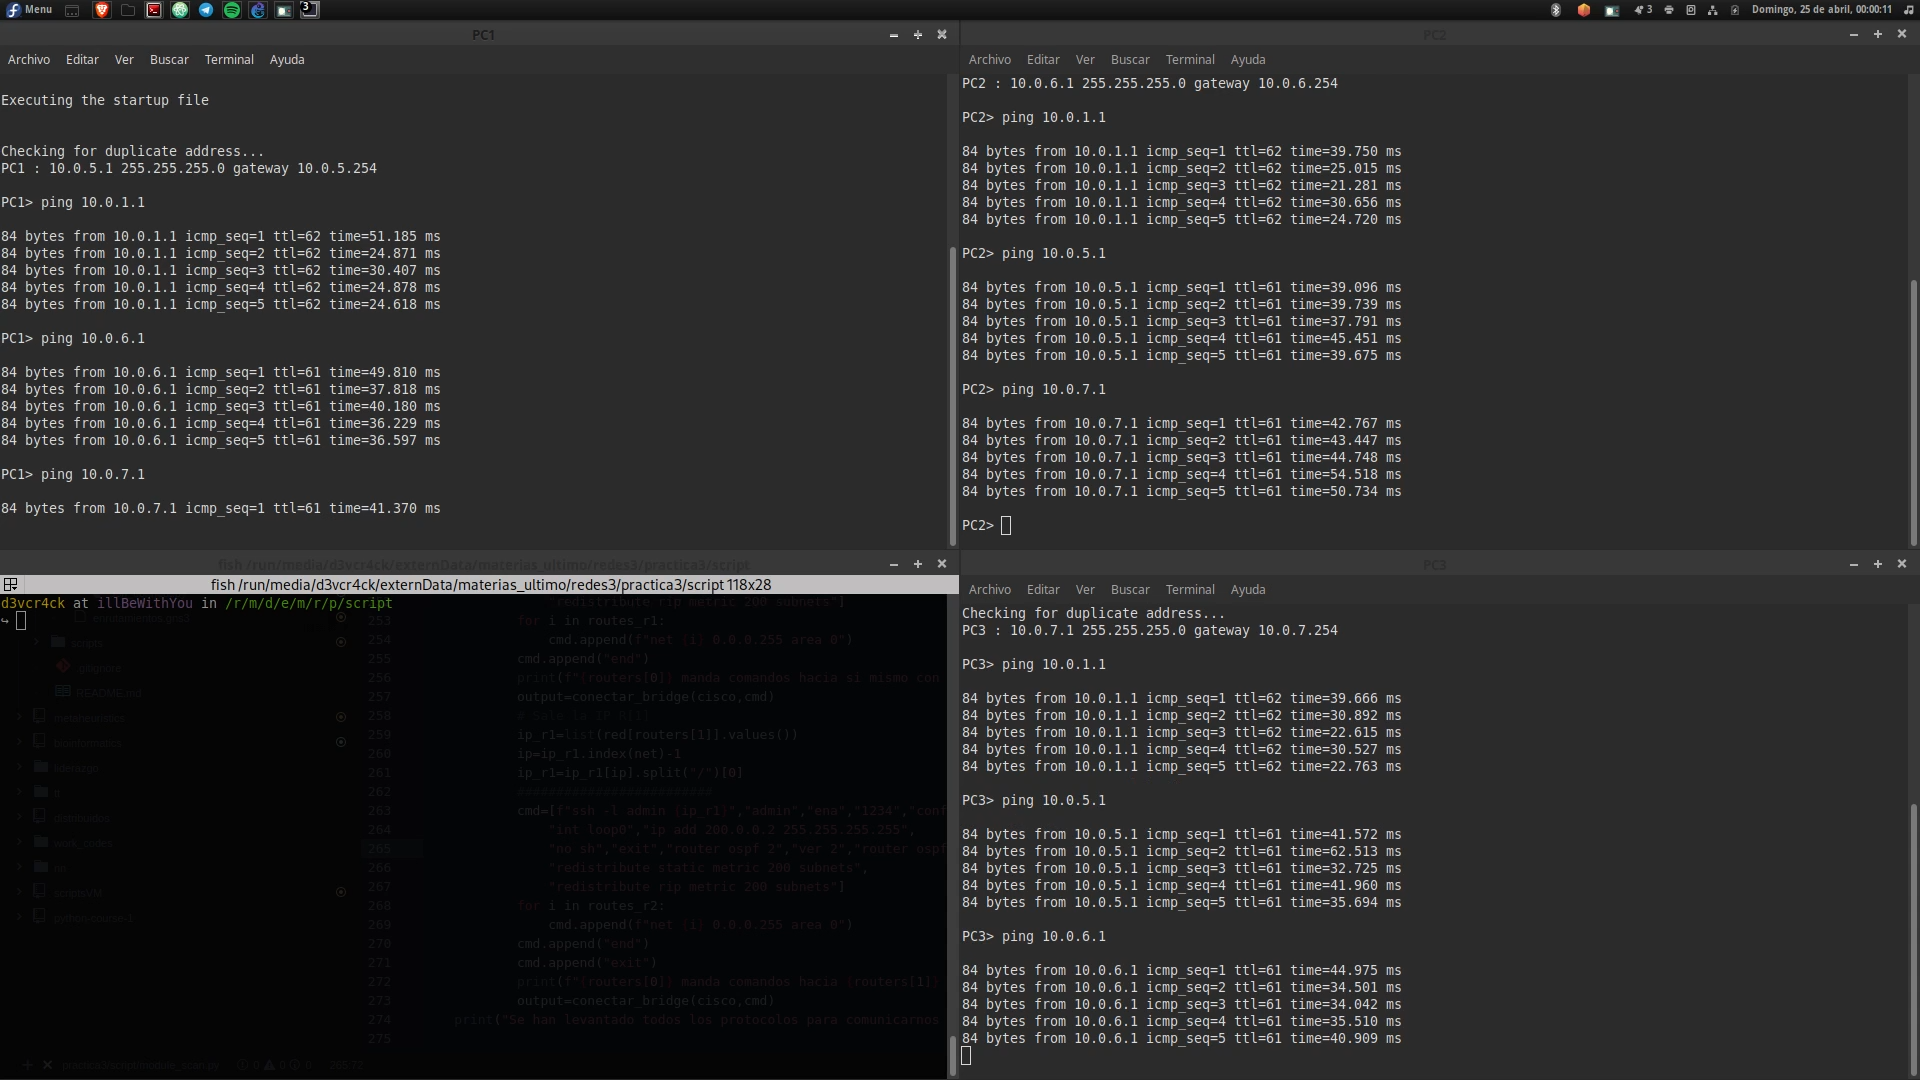
\includegraphics[scale=0.5]{imgs/4.png}\\
  \textit{Figura 4: Pings entre subredes}
\end{center}


\end{document}
